\documentclass[11pt,aspectratio=169]{beamer}
\usepackage{amsmath,amssymb,bm,graphicx,tikz}
\usetheme{default}
\setbeamertemplate{navigation symbols}{}
\setbeamertemplate{headline}{}
\setbeamertemplate{footline}{\leavevmode\hbox{%
  \begin{beamercolorbox}[wd=\paperwidth,ht=2.6ex,dp=1.1ex,right]{page number in head/foot}%
    \insertframenumber/\inserttotalframenumber\hspace{0.35cm}
  \end{beamercolorbox}}}
\setbeamertemplate{frametitle}{\vspace{0.25cm}\insertframetitle\par\vspace{0.08cm}\hrule}
\setbeamercolor{normal text}{fg=black,bg=white}
\setbeamercolor{frametitle}{fg=black,bg=white}
\setbeamercolor{structure}{fg=black}
\setbeamersize{text margin left=0.7cm,text margin right=0.7cm}
\graphicspath{{figures/}}
\newcommand{\dd}{\mathrm d}
\newcommand{\bU}{\bm U}
\newcommand{\bx}{\bm x}
\newcommand{\bM}{\bm M}
\newcommand{\bK}{\bm K}
\newcommand{\bF}{\bm F}
\newcommand{\Vzero}{\mathcal V_0}
\newcommand{\Vhzero}{\mathcal V_{h,0}}
\newcommand{\Thot}{T_{\mathrm{hot}}}
\newcommand{\Tcold}{T_{\mathrm{cold}}}

\begin{document}

\begin{frame}
\centering\vfill
{\LARGE\bfseries Transient Finite Element Methods\par}
\vspace{0.45cm}
{\Large Lecture 1: Heat Conduction and Time Discretization\par}
\vspace{0.45cm}
Prashant K. Jha\par
ME/BME 736
\vfill
\end{frame}

\begin{frame}{Lecture outline}
\begin{enumerate}
\item Heat and wave equations: boundary conditions, initial conditions, and exact solutions.
\item The heat equation in general dimension and its variational form at a fixed time.
\item Spatial finite element approximation and the coefficient equations.
\item Forward Euler, backward Euler, and the $\theta$-method.
\item Time stepping and numerical results for the heated bar.
\end{enumerate}
\medskip
We use $T(\bx,t)$ for the temperature field and $U_i(t)$ for its finite
element coefficients.
\end{frame}

\begin{frame}{Heat conduction in a bar: boundary and initial conditions}
A bar of length $L$ has an insulated lateral surface and no internal heat source.
Its ends are held at fixed temperatures $\Thot>\Tcold$.
\begin{center}
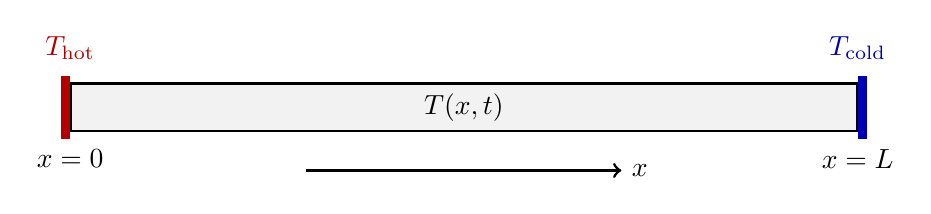
\begin{tikzpicture}[line width=1pt]
\draw[fill=gray!10] (0,0) rectangle (10,0.6);
\fill[red!70!black] (-0.12,-0.1) rectangle (0,0.7);
\fill[blue!70!black] (10,-0.1) rectangle (10.12,0.7);
\node[text=red!70!black] at (0,1.05) {$\Thot$};
\node[text=blue!70!black] at (10,1.05) {$\Tcold$};
\node at (5,0.3) {$T(x,t)$};
\node[below] at (0,-0.1) {$x=0$};
\node[below] at (10,-0.1) {$x=L$};
\draw[->] (3,-0.5) -- (7,-0.5) node[right] {$x$};
\end{tikzpicture}
\end{center}
\textbf{Boundary conditions} for $0\le t\le t_f$:
\[
T(0,t)=\Thot,\qquad T(L,t)=\Tcold.
\]
\textbf{Initial condition} for $0\le x\le L$:
\[
T(x,0)=T_0(x)=T_s(x)+A\sin(\pi x/L),\qquad
T_s(x)=\Thot+(\Tcold-\Thot)\frac{x}{L}.
\]
Here $A$ is a prescribed temperature amplitude.
Since the sine is zero at both ends, $T_0(0)=\Thot$ and $T_0(L)=\Tcold$.
\end{frame}

\begin{frame}{The heat equation and an exact solution}
Let density $\rho$, specific heat $c$, and conductivity $k$ be positive constants.
The thermal diffusivity is $\alpha=k/(\rho c)$, in $\mathrm{m^2/s}$.
The complete initial-boundary-value problem is
\[
\boxed{\begin{cases}
\rho c\,\partial_tT-k\partial_{xx}T=0,&0<x<L,\quad 0<t\le t_f,\\
T(0,t)=\Thot,\quad T(L,t)=\Tcold,&0\le t\le t_f,\\
T(x,0)=T_s(x)+A\sin(\pi x/L),&0\le x\le L.
\end{cases}}
\]
The exact solution is
\[
T_{\mathrm{exact}}(x,t)=T_s(x)
+A e^{-\frac{\alpha\pi^2}{L^2}t}\sin(\pi x/L).
\]
The linear profile $T_s$ has $T_s''=0$. For the remaining term,
\[
\rho c\,\partial_tT_{\mathrm{exact}}=k\partial_{xx}T_{\mathrm{exact}}
=-\frac{k\pi^2 A}{L^2}e^{-\frac{k\pi^2}{\rho c L^2}t}\sin(\pi x/L).
\]
\end{frame}

\begin{frame}{Heat conduction: exact temperature profiles}
Use $L=1$, $\rho c=k=1$, $\Thot=400\,\mathrm K$, $\Tcold=300\,\mathrm K$,
and $A=20\,\mathrm K$.
\centering
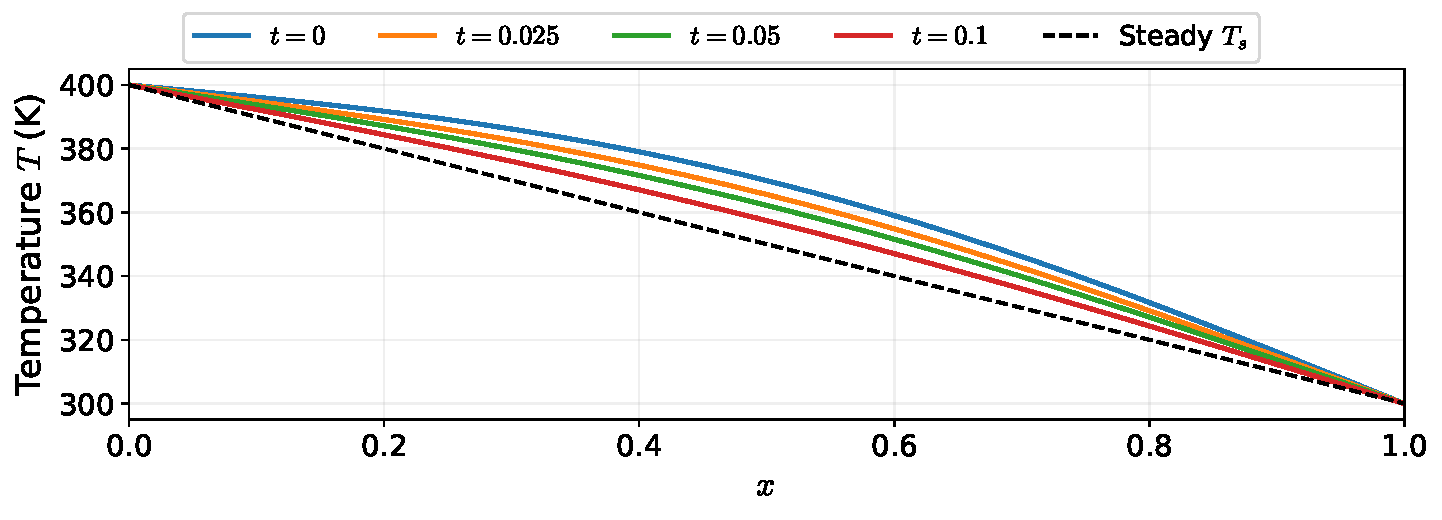
\includegraphics[width=0.91\textwidth]{exact_bar.pdf}
\par\raggedright
The end temperatures remain fixed. The initial excess temperature decays,
and $T(x,t)$ approaches the steady profile $T_s(x)=400-100x$.
\end{frame}

\begin{frame}{A vibrating bar: boundary and initial conditions}
Let $u(x,t)$ be the axial displacement of an undamped bar of length $1$.
Both ends are fixed.
\begin{center}
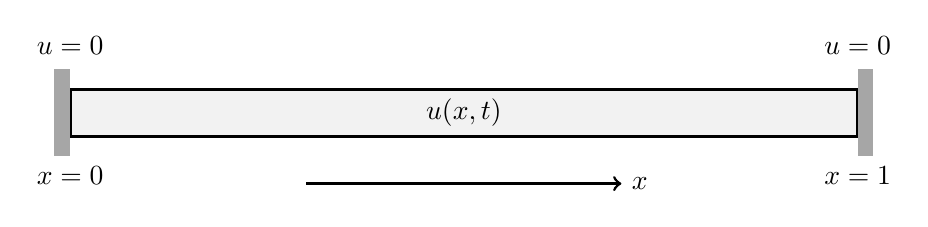
\begin{tikzpicture}[line width=1pt]
\draw[fill=gray!10] (0,0) rectangle (10,0.6);
\fill[gray!70] (-0.2,-0.25) rectangle (0,0.85);
\fill[gray!70] (10,-0.25) rectangle (10.2,0.85);
\node at (0,1.15) {$u=0$};
\node at (10,1.15) {$u=0$};
\node at (5,0.3) {$u(x,t)$};
\node[below] at (0,-0.25) {$x=0$};
\node[below] at (10,-0.25) {$x=1$};
\draw[->] (3,-0.6) -- (7,-0.6) node[right] {$x$};
\end{tikzpicture}
\end{center}
\textbf{Boundary conditions} for $0\le t\le t_f$:
\[
u(0,t)=u(1,t)=0.
\]
\textbf{Initial conditions} for $0\le x\le1$:
\[
u(x,0)=u_0(x),\qquad \partial_tu(x,0)=v_0(x).
\]
The given functions $u_0$ and $v_0$ specify the initial displacement and velocity.
\end{frame}

\begin{frame}{Example: a one-dimensional wave}
Let $u(x,t)$ be the axial displacement of an undamped bar with fixed ends.
For constant density $\rho>0$ and Young's modulus $E>0$, the wave speed is
$c_w=\sqrt{E/\rho}$. Choose the initial pulse
\[
u_0(s)=\begin{cases}
\bigl[1-100(s-\tfrac14)^2\bigr]^3,&|s-\tfrac14|<\tfrac1{10},\\
0,&\text{otherwise},
\end{cases}
\qquad s\in\mathbb R.
\]
The wave problem is
\[
\boxed{\begin{cases}
\rho\,\partial_{tt}u-E\partial_{xx}u=0,&0<x<1,\quad 0<t\le0.6/c_w,\\
u(0,t)=u(1,t)=0,&0\le t\le0.6/c_w,\\
u(x,0)=u_0(x),\quad \partial_tu(x,0)=v_0(x)=-c_wu_0'(x),&0\le x\le1.
\end{cases}}
\]
Both the initial displacement and the initial velocity are prescribed.
The exact solution is
\[
u_{\mathrm{exact}}(x,t)=u_0(x-c_wt).
\]
\end{frame}

\begin{frame}{Wave: an exact traveling pulse}
For the plots, take $E=\rho=1$. Then $c_w=1$ and $u_0(x-t)$ moves to the right.
\centering
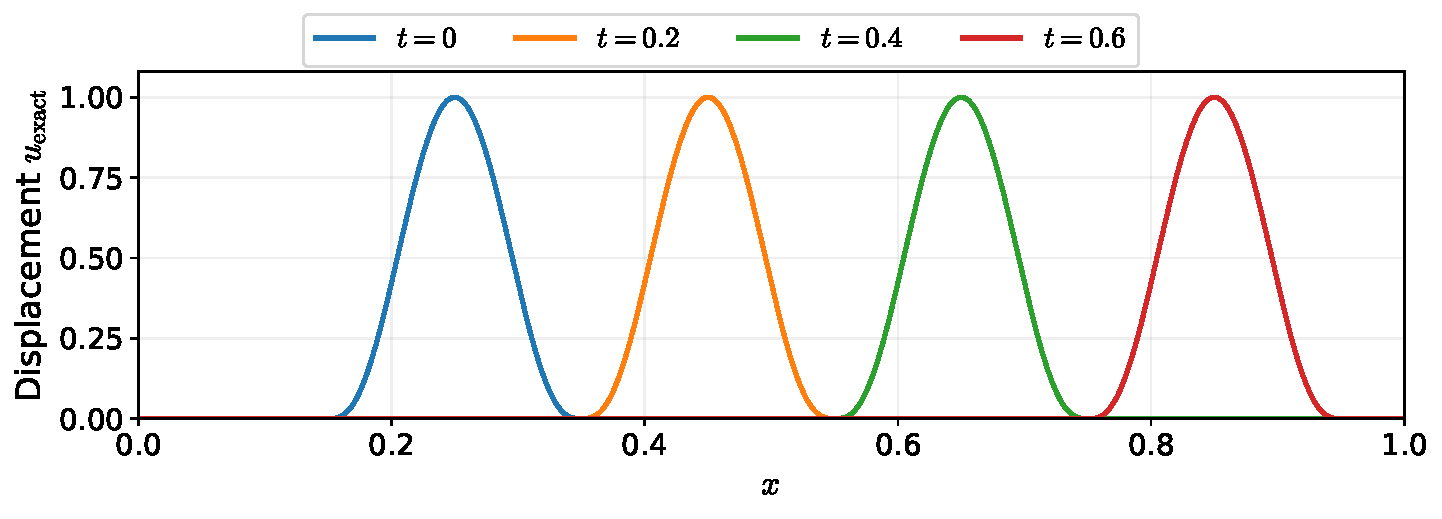
\includegraphics[width=0.91\textwidth]{exact_wave.pdf}
\par\raggedright
Differentiating $u_0(x-c_wt)$ at $t=0$ gives the prescribed velocity $-c_wu_0'(x)$.
The peak moves from $x=0.25$ to $x=0.25+t$.
Through $t=0.6$, the pulse stays inside $(0,1)$, so both endpoint values remain zero.
\end{frame}

\begin{frame}{The order of the time derivative}
\textbf{Heat: first order in time}
\[
\rho c\,\partial_tT-k\partial_{xx}T=0,\qquad T(x,0)=T_0(x).
\]
The initial temperature is prescribed.
\medskip

\textbf{Wave: second order in time}
\[
\rho\,\partial_{tt}u-E\partial_{xx}u=0,\qquad
u(x,0)=u_0(x),\quad \partial_tu(x,0)=v_0(x).
\]
Both initial displacement and initial velocity are prescribed.
\medskip

The remainder of this lecture develops the \textbf{first-order heat problem}.
The wave equation needs a time discretization for a second-order system,
or a first-order reformulation using displacement and velocity.
We do not develop its numerical solution here.
\end{frame}

\begin{frame}
\centering\vfill
{\LARGE\bfseries Variational formulation at a fixed time\par}
\vspace{0.4cm}
The heat equation on $\Omega\subset\mathbb R^d$
\vfill
\end{frame}

\begin{frame}{The heat problem in general dimension: domain and data}
Let a stationary body occupy a bounded Lipschitz domain
$\Omega\subset\mathbb R^d$, $d=1,2,3$, with position $\bx$.
Take density $\rho$, specific heat $c$, and conductivity $k$ to be positive constants.
Their ratio $\alpha=k/(\rho c)$ is the thermal diffusivity.
\medskip

Prescribe temperature on $\Gamma_T$ and normal flux on $\Gamma_q$:
\[
\partial\Omega=\overline{\Gamma_T}\cup\overline{\Gamma_q},
\qquad \Gamma_T\cap\Gamma_q=\varnothing.
\]
Their interfaces have zero boundary measure and do not affect boundary integrals.
Let $\bm n$ be the outward unit normal. The flux convention is
\[
q=k\nabla T\cdot\bm n.
\]
The physical heat-flow vector is $-k\nabla T$, so $q>0$ means heat enters the body.
The prescribed temperature $\overline T(\bx)$ is fixed in time.
\end{frame}

\begin{frame}{The heat equation: strong form, BCs, and IC}
Let $r(\bx,t)$ be the prescribed volumetric heat supply and
$T_0(\bx)$ the initial temperature. Solve
\[
\boxed{\begin{aligned}
\rho c\,\partial_tT-\nabla\!\cdot(k\nabla T)&=r(\bx,t)
&&\text{in }\Omega,\quad 0<t\le t_f,\\
T(\bx,t)&=\overline T(\bx)
&&\text{on }\Gamma_T,\quad 0\le t\le t_f,\\
k\nabla T(\bx,t)\cdot\bm n&=q(\bx,t)
&&\text{on }\Gamma_q,\quad 0<t\le t_f,\\
T(\bx,0)&=T_0(\bx)
&&\text{in }\Omega.
\end{aligned}}
\]
The middle two equations are the \textbf{boundary conditions}.
The last equation is the \textbf{initial condition}.
\medskip

For a classical solution, the data agree at the initial time:
$T_0=\overline T$ on $\Gamma_T$.
The bar example has $\Omega=(0,L)$ with both endpoint temperatures prescribed.
\end{frame}

\begin{frame}{Multiply by a spatial test function}
Fix a time $t$ and write $\dot T=\partial_tT$. Start with
\[
\rho c\,\dot T-\nabla\!\cdot(k\nabla T)=r.
\]
Choose a smooth spatial test function $v(\bx)$ with $v=0$ on $\Gamma_T$.
Multiplication by $v$ and integration over $\Omega$ give
\[
\int_\Omega\rho c\,\dot T\,v\,\dd\bx
-\int_\Omega\nabla\!\cdot(k\nabla T)v\,\dd\bx
=\int_\Omega rv\,\dd\bx.
\]
All fields are evaluated at this same time $t$.
There is no integration in time in this step.
\end{frame}

\begin{frame}{Integration by parts in space}
Apply integration by parts to the second integral:
\[
\begin{aligned}
-\int_\Omega\nabla\!\cdot(k\nabla T)v\,\dd\bx
={}&\int_\Omega k\nabla T\cdot\nabla v\,\dd\bx\\
&-\int_{\partial\Omega}(k\nabla T\cdot\bm n)v\,\dd s.
\end{aligned}
\]
Substitute into the integrated equation:
\[
\begin{aligned}
\int_\Omega\rho c\,\dot T\,v\,\dd\bx
+\int_\Omega k\nabla T\cdot\nabla v\,\dd\bx
={}&\int_\Omega rv\,\dd\bx\\
&+\int_{\partial\Omega}(k\nabla T\cdot\bm n)v\,\dd s.
\end{aligned}
\]
The boundary integral still includes both $\Gamma_T$ and $\Gamma_q$.
\end{frame}

\begin{frame}{Use the boundary conditions in the boundary integral}
Split the boundary integral from the previous identity:
\[
\begin{aligned}
\int_{\partial\Omega}(k\nabla T\cdot\bm n)v\,\dd s
={}&\underbrace{\int_{\Gamma_T}(k\nabla T\cdot\bm n)v\,\dd s}_{0\text{ because }v=0\text{ on }\Gamma_T}\\
&+\underbrace{\int_{\Gamma_q}(k\nabla T\cdot\bm n)v\,\dd s}_{\int_{\Gamma_q}qv\,\dd s}.
\end{aligned}
\]
Substitution gives
\[
\boxed{\begin{aligned}
\int_\Omega\rho c\,\dot T\,v\,\dd\bx
+\int_\Omega k\nabla T\cdot\nabla v\,\dd\bx
={}&\int_\Omega rv\,\dd\bx\\
&+\int_{\Gamma_q}qv\,\dd s.
\end{aligned}}
\]
\end{frame}

\begin{frame}{Spatial trial and test spaces}
At each time $t$, use the spatial trial space
\[
\mathcal U_{\overline T}
=\{S\in H^1(\Omega):S=\overline T\text{ on }\Gamma_T\}
\]
and the spatial test space
\[
\Vzero=\{v\in H^1(\Omega):v=0\text{ on }\Gamma_T\}.
\]
The trial functions satisfy the prescribed temperatures.
The test functions vanish on $\Gamma_T$, but need not vanish on $\Gamma_q$.
\medskip

For this derivation, assume also that the solution is differentiable in time
with $\dot T(\cdot,t)\in L^2(\Omega)$.
Take $r(\cdot,t)\in L^2(\Omega)$, $q(\cdot,t)\in L^2(\Gamma_q)$,
and assume $\overline T$ is the boundary value of an $H^1(\Omega)$ function.
\end{frame}

\begin{frame}{The spatial variational problem}
Define the bilinear forms $m,a_T$ and the linear functional $\ell_T$:
\[
\begin{aligned}
m(S,v)&=\int_\Omega\rho c\,Sv\,\dd\bx,\\
a_T(S,v)&=\int_\Omega k\nabla S\cdot\nabla v\,\dd\bx,\\
\ell_T(t;v)&=\int_\Omega r(\bx,t)v\,\dd\bx
+\int_{\Gamma_q}q(\bx,t)v\,\dd s.
\end{aligned}
\]
For each $t>0$, find $T(\cdot,t)\in\mathcal U_{\overline T}$ such that
\[
\boxed{m(\dot T,v)+a_T(T,v)=\ell_T(t;v)
\qquad\forall v\in\Vzero.}
\]
The evolution starts from $T(\cdot,0)=T_0$.
Time is still continuous.
\end{frame}

\begin{frame}
\centering\vfill
{\LARGE\bfseries Finite element approximation in space\par}
\vspace{0.4cm}
Fixed basis functions and time-dependent coefficients
\vfill
\end{frame}

\begin{frame}{The mesh, basis, and temperature coefficients}
Mesh $\Omega$ with elements $\mathcal K_e$.
Let $\mathcal V_h$ be a continuous Lagrange finite element space on this fixed mesh,
with nodes $\bx_1,\ldots,\bx_{N_n}$ and nodal basis functions satisfying
\[
\phi_i(\bx_j)=\delta_{ij},\qquad i,j=1,\ldots,N_n.
\]
Approximate the temperature by
\[
\boxed{T_h(\bx,t)=\sum_{j=1}^{N_n}U_j(t)\phi_j(\bx).}
\]
The field is $T_h$; the $U_j(t)$ are its coefficients.
They vary with time, while the mesh and basis functions do not.
\medskip

Prescribe the coefficients at nodes on $\Gamma_T$:
\[
U_i(t)=\overline T(\bx_i),\qquad \bx_i\in\Gamma_T.
\]
All remaining coefficients are \textbf{free}: they are unknown functions of time.
\end{frame}

\begin{frame}{Differentiate the finite element temperature}
Seek differentiable coefficient functions $U_j(t)$.
Starting from $T_h=\sum_jU_j(t)\phi_j(\bx)$, the product rule gives
\[
\partial_tT_h
=\sum_{j=1}^{N_n}\dot U_j(t)\phi_j(\bx)
+\sum_{j=1}^{N_n}U_j(t)\partial_t\phi_j(\bx).
\]
The basis is independent of time, so $\partial_t\phi_j=0$:
\[
\boxed{\dot T_h(\bx,t)=\sum_{j=1}^{N_n}\dot U_j(t)\phi_j(\bx).}
\]
Each $\phi_j$ is square-integrable, so this finite sum also belongs to $L^2(\Omega)$.
\medskip

For time-independent prescribed temperatures,
$\dot U_i(t)=0$ at nodes on $\Gamma_T$.
\end{frame}

\begin{frame}{Substitute into the variational equation}
The discrete test space is $\Vhzero=\mathcal V_h\cap\Vzero$.
The basis functions associated with free nodes vanish on $\Gamma_T$ and
are admissible test functions.
\medskip

For each free node $i$, set $v_h=\phi_i$ and substitute $T_h,\dot T_h$:
\[
m\left(\sum_{j=1}^{N_n}\dot U_j\phi_j,\phi_i\right)
+a_T\left(\sum_{j=1}^{N_n}U_j\phi_j,\phi_i\right)
=\ell_T(t;\phi_i).
\]
Because $m$ and $a_T$ are bilinear, we can take each coefficient outside its spatial integral:
\[
\boxed{
\sum_{j=1}^{N_n}m(\phi_j,\phi_i)\dot U_j
+\sum_{j=1}^{N_n}a_T(\phi_j,\phi_i)U_j
=\ell_T(t;\phi_i).}
\]
The sums include \emph{all} nodes, including those with prescribed temperatures.
\end{frame}

\begin{frame}{The assembled matrices and load vector}
For all $i,j=1,\ldots,N_n$, assemble
\[
\begin{aligned}
M_{ij}&=m(\phi_j,\phi_i)=\int_\Omega\rho c\,\phi_j\phi_i\,\dd\bx,\\
K_{ij}&=a_T(\phi_j,\phi_i)=\int_\Omega k\nabla\phi_j\cdot\nabla\phi_i\,\dd\bx,\\
F_i(t)&=\ell_T(t;\phi_i)=\int_\Omega r(\bx,t)\phi_i\,\dd\bx
+\int_{\Gamma_q}q(\bx,t)\phi_i\,\dd s.
\end{aligned}
\]
With the full coefficient vector $\bU=(U_1,\ldots,U_{N_n})^T$,
the tested equations are the free rows of
\[
\boxed{\bM\dot{\bU}+\bK\bU=\bF(t).}
\]
$\bM$ is the \textbf{mass matrix}; it comes from the time-derivative term.
$\bK$ is the stiffness matrix.
\end{frame}

\begin{frame}{Free and prescribed coefficient equations}
The variational equation supplies one equation for each free coefficient:
\[
\sum_{j=1}^{N_n}M_{ij}\dot U_j+\sum_{j=1}^{N_n}K_{ij}U_j=F_i(t),
\qquad i\text{ free}.
\]
At a prescribed-temperature node, $\phi_i$ does not vanish on $\Gamma_T$ and
is not an admissible test function. Instead, impose
\[
\boxed{U_i(t)=\overline T(\bx_i),\qquad \bx_i\in\Gamma_T.}
\]
Assemble the matrices for all nodes, then enforce these values and solve the
free equations.
\medskip

Free nodes include interior nodes and nodes on $\Gamma_q$.
After accounting for the prescribed values, their coefficients
satisfy a system of first-order ODEs.
\end{frame}

\begin{frame}{Element contributions in any dimension}
On an element $\mathcal K_e$, let $\phi_a^e$ be the local shape functions.
The element matrices are
\[
M^e_{ab}=\int_{\mathcal K_e}\rho c\,\phi_b^e\phi_a^e\,\dd\bx,
\qquad K^e_{ab}=\int_{\mathcal K_e}k\nabla\phi_b^e\cdot\nabla\phi_a^e\,\dd\bx.
\]
Source and prescribed-flux contributions give
\[
F_a^e(t)=\int_{\mathcal K_e}r(\bx,t)\phi_a^e\,\dd\bx
+\int_{\partial\mathcal K_e\cap\Gamma_q}q(\bx,t)\phi_a^e\,\dd s.
\]
Use the connectivity $I^e$ from Chapters 5 and 6 to assemble
$\bM^e$, $\bK^e$, and $\bF^e$ into the global arrays.
The spatial assembly is unchanged by the subsequent time discretization.
\end{frame}

\begin{frame}{Initial coefficient values}
Before advancing the ODEs, specify their initial values.
For continuous $T_0$ compatible with the prescribed boundary values, use nodal interpolation:
\[
U_i(0)=T_0(\bx_i),\qquad i=1,\ldots,N_n.
\]
The full initial vector is $\bU^0=(U_1(0),\ldots,U_{N_n}(0))^T$.
The superscript $0$ denotes the initial time.
At prescribed-temperature nodes, compatibility gives
\[
U_i^0=T_0(\bx_i)=\overline T(\bx_i),\qquad \bx_i\in\Gamma_T.
\]
\medskip

We now have a spatial approximation and its initial values.
The next step is to approximate its evolution in time.
\end{frame}

\begin{frame}
\centering\vfill
{\LARGE\bfseries Time discretization\par}
\vspace{0.4cm}
First a scalar ODE, then the finite element coefficient equations
\vfill
\end{frame}

\begin{frame}{A time grid for a first-order ODE}
Consider
\[
\dot y(t)=f(t,y(t)),\qquad y(0)=y_0.
\]
Choose $t_n=n\Delta t$, with $\Delta t>0$, and let
$y^n$ approximate $y(t_n)$.
At a time step, $y^n$ is known and $y^{n+1}$ must be found.
\medskip

The difference quotient across $[t_n,t_{n+1}]$ is
\[
\frac{y^{n+1}-y^n}{\Delta t}.
\]
We can use it to approximate the derivative at the old endpoint $t_n$
or the new endpoint $t_{n+1}$.
These two choices give forward Euler and backward Euler, respectively.
\end{frame}

\begin{frame}{Forward Euler: use the derivative at the old time}
Approximate the derivative at $t_n$:
\[
\dot y(t_n)\approx\frac{y^{n+1}-y^n}{\Delta t}.
\]
The ODE gives $\dot y(t_n)=f(t_n,y(t_n))$.
Using $y^n$ for the old solution value gives the scheme
\[
\frac{y^{n+1}-y^n}{\Delta t}=f(t_n,y^n),
\qquad
\boxed{y^{n+1}=y^n+\Delta t\,f(t_n,y^n).}
\]
The right-hand side contains only known quantities.
\medskip

For $\dot y=-y$, $y^0=1$, and $\Delta t=0.5$,
\[
y^1=1+0.5(-1)=0.5.
\]
\end{frame}

\begin{frame}{Backward Euler: use the derivative at the new time}
Approximate the derivative at $t_{n+1}$:
\[
\dot y(t_{n+1})\approx\frac{y^{n+1}-y^n}{\Delta t}.
\]
The ODE gives $\dot y(t_{n+1})=f(t_{n+1},y(t_{n+1}))$.
Using the unknown new value gives
\[
\frac{y^{n+1}-y^n}{\Delta t}=f(t_{n+1},y^{n+1}),
\qquad
\boxed{y^{n+1}=y^n+\Delta t\,f(t_{n+1},y^{n+1}).}
\]
The new value appears on both sides, so this equation must be solved.
For $\dot y=-y$, $y^0=1$, and $\Delta t=0.5$,
\[
y^1=1-0.5y^1,\qquad 1.5y^1=1,\qquad y^1=\frac23.
\]
\end{frame}

\begin{frame}{One Euler step for the same ODE}
For $\dot y=-y$, $y(0)=1$, the exact solution is $e^{-t}$.
Both methods use $\Delta t=0.5$.
\centering
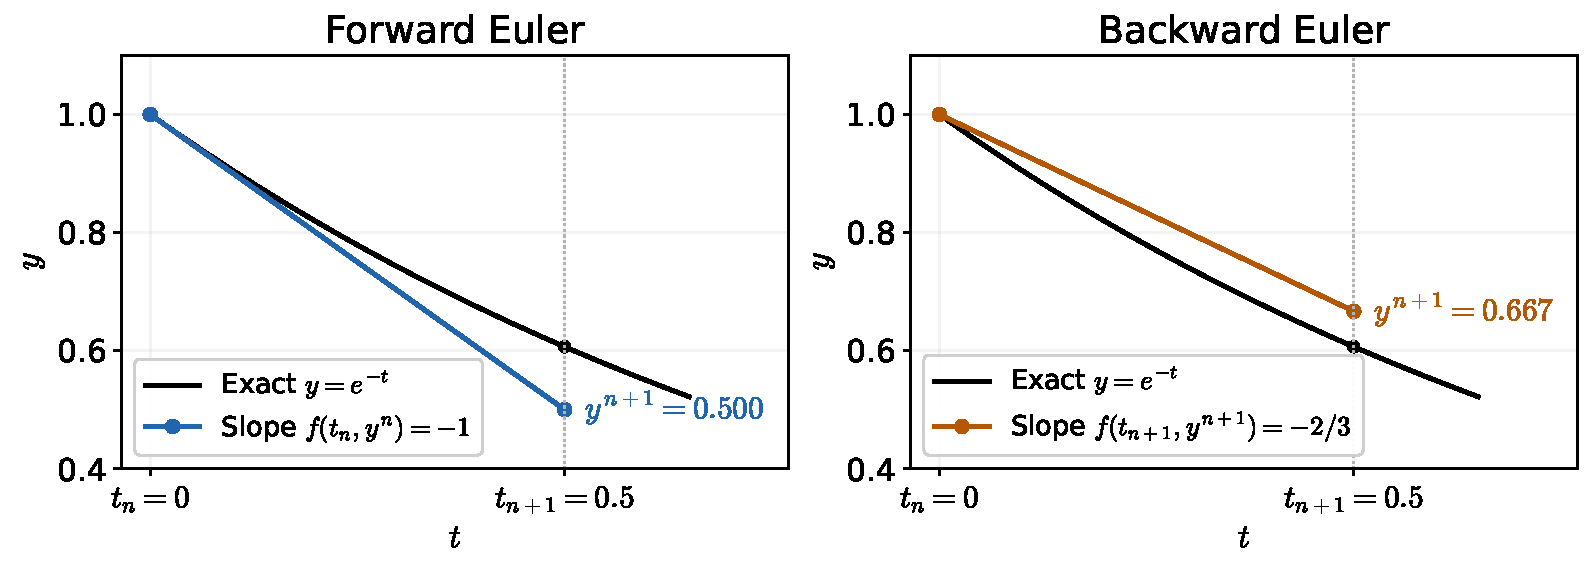
\includegraphics[width=0.96\textwidth]{euler_slopes.pdf}
\par\raggedright
The difference quotient is the slope of the straight segment.
Forward Euler uses the old endpoint rate; backward Euler uses the new endpoint rate.
\end{frame}

\begin{frame}{The $\theta$-method: weight the endpoint rates}
Combine the old and new endpoint evaluations:
\[
\boxed{\frac{y^{n+1}-y^n}{\Delta t}
=(1-\theta)f(t_n,y^n)+\theta f(t_{n+1},y^{n+1}),
\qquad 0\le\theta\le1.}
\]
\begin{center}
\begin{tabular}{cl}
$\theta$ & Method\\ \hline
$0$ & Forward Euler\\
$1$ & Backward Euler\\
$1/2$ & Trapezoidal rule
\end{tabular}
\end{center}
For $\theta=1/2$, average the two endpoint rates.
For the heat equation, this gives Crank--Nicolson.
\medskip

The weighting is between endpoint \emph{values of $f$}.
It is not an evaluation of $f$ at one intermediate time.
\end{frame}

\begin{frame}{Backward Euler for the finite element equations}
Return to the free rows of $\bM\dot{\bU}+\bK\bU=\bF(t)$.
Write $\bU^n\approx\bU(t_n)$ and $\bF^n=\bF(t_n)$.
Apply backward Euler:
\[
\left[\bM\frac{\bU^{n+1}-\bU^n}{\Delta t}
+\bK\bU^{n+1}\right]_i=F_i(t_{n+1}),
\qquad i\text{ free}.
\]
Multiply by $\Delta t$ and collect the new coefficient values:
\[
\boxed{
\bigl[(\bM+\Delta t\,\bK)\bU^{n+1}\bigr]_i
=\bigl[\bM\bU^n+\Delta t\,\bF^{n+1}\bigr]_i.}
\]
At prescribed-temperature nodes, impose
\[
U_i^{n+1}=\overline T(\bx_i),\qquad \bx_i\in\Gamma_T.
\]
These equations determine the temperature coefficients at the new time.
\end{frame}

\begin{frame}{The $\theta$-method for the finite element equations}
Weight the old and new values of the conduction and source terms.
For each free row $i$,
\[
\left[\bM\frac{\bU^{n+1}-\bU^n}{\Delta t}
+(1-\theta)\bK\bU^n+\theta\bK\bU^{n+1}\right]_i
=\bigl[(1-\theta)\bF^n+\theta\bF^{n+1}\bigr]_i.
\]
Multiply by $\Delta t$ and rearrange. The assembled update is
\[
\boxed{\begin{aligned}
(\bM+\theta\Delta t\,\bK)\bU^{n+1}
={}&[\bM-(1-\theta)\Delta t\,\bK]\bU^n\\
&+\Delta t[(1-\theta)\bF^n+\theta\bF^{n+1}].
\end{aligned}}
\tag{1}\label{eq:theta-update}
\]
Use its free rows and replace the prescribed-temperature rows by
$U_i^{n+1}=\overline T(\bx_i)$.
\end{frame}

\begin{frame}{The time-stepping algorithm}
\textbf{Initialize}

Assemble the full $\bM,\bK$ and set $U_i^0=T_0(\bx_i)$.
Choose $\theta,\Delta t,N_t$ with $N_t\Delta t=t_f$. Form
\[
\bm B=\bM+\theta\Delta t\,\bK,\qquad
\bm C=\bM-(1-\theta)\Delta t\,\bK.
\]
\textbf{For $n=0,\ldots,N_t-1$}
\begin{enumerate}
\item Evaluate $\bF^n=\bF(t_n)$ and $\bF^{n+1}=\bF(t_{n+1})$.
\item Form
\[
\bm b^n=\bm C\bU^n+\Delta t[(1-\theta)\bF^n+\theta\bF^{n+1}].
\]
\item Impose $U_i^{n+1}=\overline T(\bx_i)$ at nodes on $\Gamma_T$.
Solve the free rows of $\bm B\bU^{n+1}=\bm b^n$.
\item Reconstruct $T_h^{n+1}(\bx)=\sum_jU_j^{n+1}\phi_j(\bx)$ and save the result.
\end{enumerate}
\end{frame}

\begin{frame}{One-dimensional linear elements for the bar example}
For the worked calculation, return to $\Omega=(0,L)$.
On $\mathcal K_e=[x_e,x_{e+1}]$, set $h_e=x_{e+1}-x_e$ and use
\[
\phi_1^e(x)=\frac{x_{e+1}-x}{h_e},
\qquad \phi_2^e(x)=\frac{x-x_e}{h_e}.
\]
The general element formulas become
\[
M^e_{ab}=\int_{\mathcal K_e}\rho c\,\phi_b^e\phi_a^e\,\dd x,
\qquad K^e_{ab}=\int_{\mathcal K_e}k(\phi_b^e)'(\phi_a^e)'\,\dd x.
\]
For example,
$\int_{\mathcal K_e}(\phi_1^e)^2\,\dd x=h_e/3$ and
$\int_{\mathcal K_e}\phi_1^e\phi_2^e\,\dd x=h_e/6$.
Hence
\[
\boxed{\bM^e=\frac{\rho c\,h_e}{6}\begin{bmatrix}2&1\\1&2\end{bmatrix},
\qquad
\bK^e=\frac{k}{h_e}\begin{bmatrix}1&-1\\-1&1\end{bmatrix}.}
\]
Both endpoints have prescribed temperatures, so this example has no flux-boundary load.
\end{frame}

\begin{frame}{Return to the heated bar}
Use $L=\rho c=k=1$, $r=0$, $\Thot=400$, and $\Tcold=300$.
With four linear elements, the five nodes are
\[
x_1=0,\quad x_2=\tfrac14,\quad x_3=\tfrac12,\quad
x_4=\tfrac34,\quad x_5=1.
\]
The finite element temperature is
\[
T_h(x,t)=\sum_{j=1}^{5}U_j(t)\phi_j(x)
=400\phi_1(x)+\sum_{j=2}^4U_j(t)\phi_j(x)+300\phi_5(x).
\]
Only $U_2,U_3,U_4$ are unknown; the endpoint coefficients stay fixed.
\medskip

Interpolate the initial condition $T_0(x)=400-100x+20\sin(\pi x)$:
\[
\bU^0=(400,\ 375+10\sqrt2,\ 370,\ 325+10\sqrt2,\ 300)^T.
\]
We will compare the computed temperatures with
$T_{\mathrm{exact}}(x,t)=400-100x+20e^{-\pi^2t}\sin(\pi x)$.
\end{frame}

\begin{frame}{The full assembled matrices for five nodes}
With $h=1/4$, assemble all four elements before enforcing the endpoint values:
\[
\bM=\frac1{24}
\begin{bmatrix}
2&1&0&0&0\\
1&4&1&0&0\\
0&1&4&1&0\\
0&0&1&4&1\\
0&0&0&1&2
\end{bmatrix},
\qquad
\bK=4
\begin{bmatrix}
1&-1&0&0&0\\
-1&2&-1&0&0\\
0&-1&2&-1&0\\
0&0&-1&2&-1\\
0&0&0&-1&1
\end{bmatrix}.
\]
There is no source, so $\bF=\bm0$.
Use rows $2,3,4$ for the temperature evolution and impose $U_1=400$, $U_5=300$.
\end{frame}

\begin{frame}{Crank--Nicolson: the prescribed-temperature terms}
Take $\theta=1/2$ and $\Delta t=0.02$ in Equation~\eqref{eq:theta-update}.
Multiply both sides by $24$. Row $2$ is
\[
0.04U_1^{n+1}+5.92U_2^{n+1}+0.04U_3^{n+1}
=1.96U_1^n+2.08U_2^n+1.96U_3^n.
\]
Insert $U_1^{n+1}=U_1^n=400$ and move the known term to the right:
\[
5.92U_2^{n+1}+0.04U_3^{n+1}
=2.08U_2^n+1.96U_3^n+\underbrace{(1.96-0.04)400}_{768}.
\]
Row $4$ similarly receives $(1.96-0.04)300=576$ from the cold end.
Row $3$ has no endpoint terms because its basis function does not touch either end.
\end{frame}

\begin{frame}{Crank--Nicolson: one numerical time step}
The three interior equations, with the endpoint terms included, are
\[
\begin{bmatrix}
5.92&0.04&0\\0.04&5.92&0.04\\0&0.04&5.92
\end{bmatrix}
\begin{bmatrix}U_2^{n+1}\\U_3^{n+1}\\U_4^{n+1}\end{bmatrix}
=
\begin{bmatrix}
2.08&1.96&0\\1.96&2.08&1.96\\0&1.96&2.08
\end{bmatrix}
\begin{bmatrix}U_2^{n}\\U_3^{n}\\U_4^{n}\end{bmatrix}
+\begin{bmatrix}768\\0\\576\end{bmatrix}.
\]
Insert the known initial coefficients and solve:
\[
\bU^1\approx(400,\ 386.481,\ 366.236,\ 336.481,\ 300)^T.
\]
Repeat five steps in total to reach $t=0.1$.
At every step the field is $T_h^n(x)=\sum_{j=1}^5U_j^n\phi_j(x)$.
\end{frame}

\begin{frame}{Computed temperatures and the exact solution}
Use $\theta=1/2$ on both meshes.
\centering
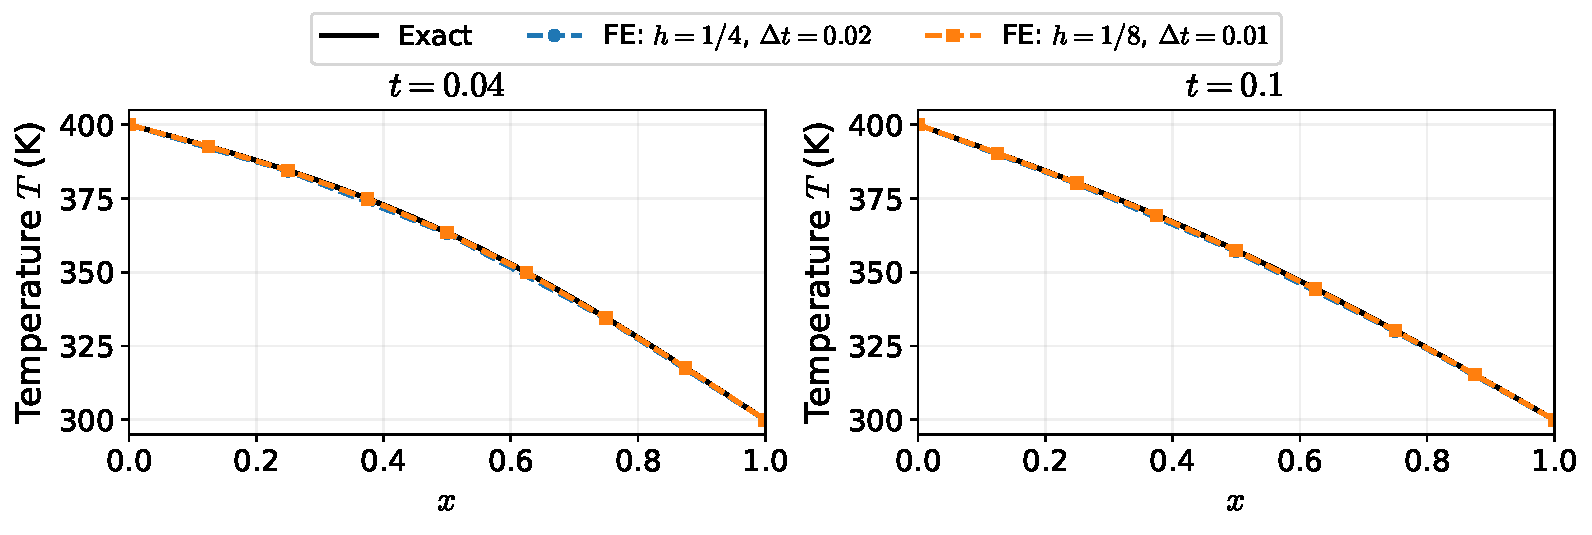
\includegraphics[width=0.96\textwidth]{bar_temperatures.pdf}
\par\raggedright
Symbols show computed nodal temperatures. The straight segments form $T_h^n$.
The refined computation halves both the element length and the time step.
\end{frame}

\begin{frame}{Refine space and time separately}
At the same final time $t_f=0.1$, measure
\[
E=\left(\int_0^1[T_h^{N_t}(x)-T_{\mathrm{exact}}(x,t_f)]^2\,\dd x\right)^{1/2}.
\]
\centering
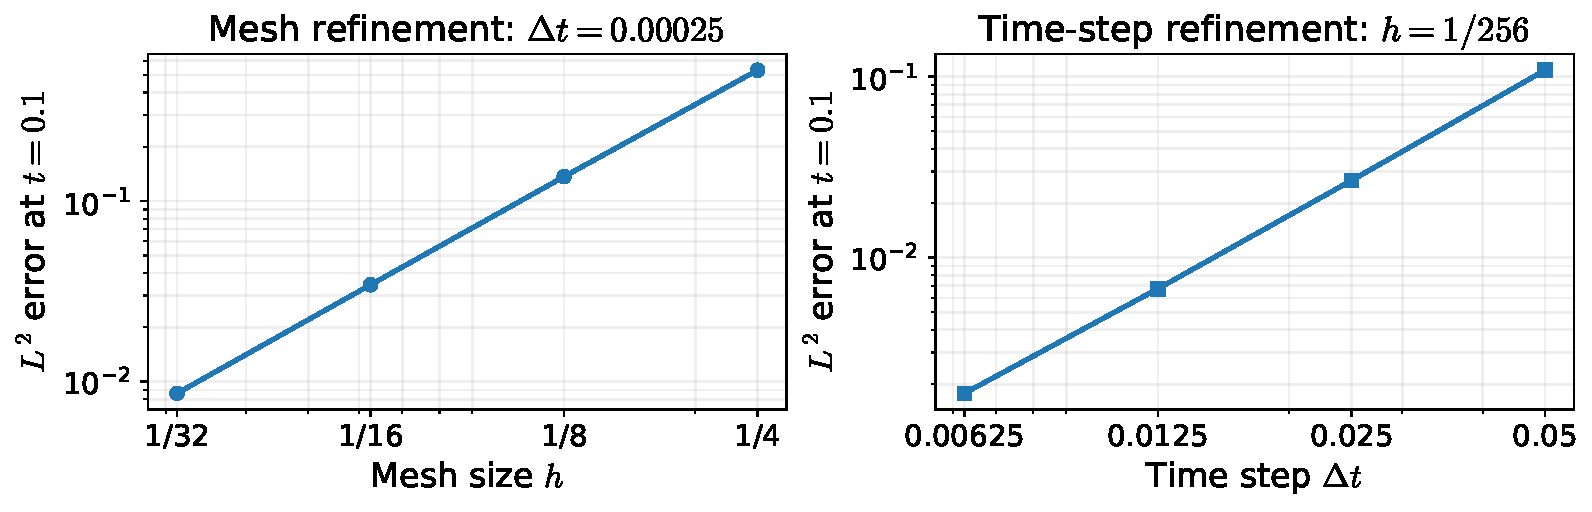
\includegraphics[width=0.96\textwidth]{bar_errors.pdf}
\par\raggedright
Left: keep $\Delta t$ small and refine $h$.
Right: keep $h$ small and reduce $\Delta t$.
\end{frame}

\begin{frame}{Summary}
\begin{itemize}
\item At a fixed time, the heat problem has a spatial variational formulation.
The initial condition determines where its evolution starts.
\item The finite element basis is fixed. Its temperature coefficients $U_i(t)$ vary with time.
\item Spatial discretization gives the free rows of
$\bM\dot{\bU}+\bK\bU=\bF$, together with prescribed-temperature equations.
\item Forward Euler uses the old endpoint rate; backward Euler uses the new one.
The $\theta$-method weights both rates.
\item Time stepping produces a sequence of linear systems and temperature fields.
Mesh size $h$ and time step $\Delta t$ control different approximations.
\end{itemize}
\end{frame}

\begin{frame}{References}
\begin{itemize}
\item Book, Chapter 4: heat equation and its variational formulation.
Chapters 5 and 6: finite element basis functions, element matrices, and assembly.
\item Larson and Bengzon, \emph{The Finite Element Method: Theory,
Implementation, and Practice}, 2010 lecture notes, Chapter 5,
pp.~95--101: spatial finite element approximation and Euler/Crank--Nicolson time stepping.
\item Arnold, \emph{Lecture Notes on Numerical Analysis of Partial
Differential Equations}, Chapter 1, Section 1.2: wave equation.
Chapter 5, Sections 1 and 3: heat-equation time stepping and finite elements.
\item \href{https://petsc.org/release/manualpages/TS/TSTHETA/}{PETSc: TSTHETA},
endpoint formulation: the weighted-endpoint convention used here.
\end{itemize}
\end{frame}

\end{document}
